\section{Classification of Self-Adaptive Systems}
\label{ch:SASClassification}

There are different approaches on how to classify and describe \acrlong{sas}[s] which all focus on different usages.
The three approaches that will be highlighted by this paper are:
\begin{itemize}[nosep]
    \item FORMS from Weyns et al., 2012 \cite*{FORMS}
    \item Berns and Ghosh, 2009 definition of self-* properties \cite*{DissectingSelfProperties}
    \item Krupitzer's et al., 2015 taxonomy for \acrlong{sas}[s] \cite*{SurveyOnEngineeringApproaches}
\end{itemize} 
These approaches contain ideas that will be used to construct the classification for
Optimization Approaches for \acrlong{sas}[s] in the next chapter.

%% FORMS
% - reflection
\begin{figure*}[b!]
    \centering
    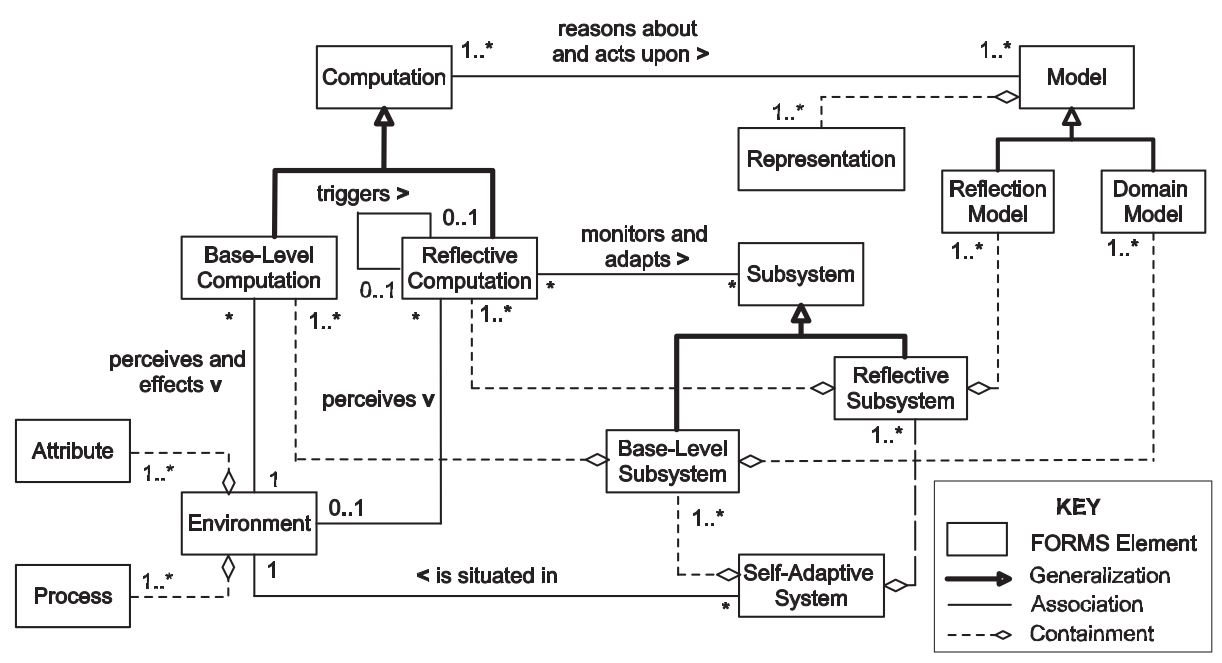
\includegraphics[width=\textwidth]{images/FORMS.png}
    \caption{FORMS primitives by Weyns et al., 2012 \cite*{FORMS}}
    \label{fig:FORMS}
\end{figure*}
\noindent In their 2012 paper FORMS \cite{FORMS} Weyns et al. propose a formal reference model for describing \acrlong{sas}[s].
The goal of FORMS is to provide a well defined basis for talking and reasoning about \acrlong{sas}[s].
This is achieved by providing a definition of FORMS which classifies \acrlong{sas}[s] using Z notation.
By composing a Self-Adaptive System from different levels of components called subsystems,
where each level can adapt the level beneath, FORMS models the self-adaptive process using reflection.
The bottom level is populated by base components and domain models.
On top of these base components are reflective components and reflection models.
The relation between these component or primitives is depicted in Figure \ref{fig:FORMS}.

\noindent The concept of different layers of reflection will be useful later to distinguish
Optimization Approaches for \acrlong{sas}[s] from \acrlong{sas}[s].

%% self-* properties
\begin{figure*}[t!]
    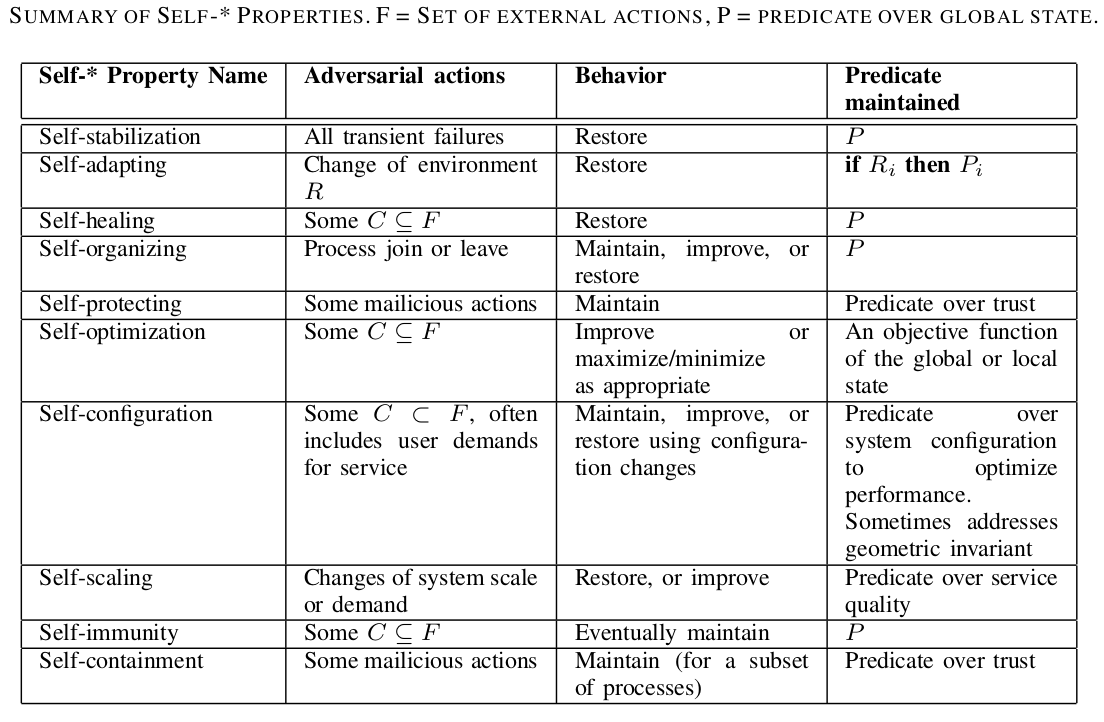
\includegraphics[width=\textwidth]{images/SelfProperties.png}
    \caption{self-* properties by Berns and Ghosh, 2009 \cite*{DissectingSelfProperties}}
    \label{fig:SelfProperties}
\end{figure*}
\noindent Although some of the first papers on \acrlong{sas}[s], for example, 
"The Vision of Autonomic Computing" by Kephart and Chess \cite*{VisionOfAutonomicComputing} focused on self-adaptation,
there are other aspects of software systems that can benefit from the ideas introduced by \acrlong{sas}[s].
Berns and Ghosh, 2009 \cite*{DissectingSelfProperties} identified and described such aspects which they call self-* properties.
These self-properties can be seen in Figure \ref{fig:SelfProperties}.
They are useful to:
\begin{itemize}[nosep]
    \item Communicate the abilities and goals of a system.
    \item Establish well-defined goals for the system.
\end{itemize}

\noindent These self-* properties show that there are aspects besides the management of software which can benefit from the ideas of Self-Adaptation.
This will be useful for the proposed classification as it gives a clear setting for the Optimization Approaches to work within.
% TODO: OA for SAS should only focus on Self-Adaptation, other abilities should be ignored.

\begin{figure*}[t!]
    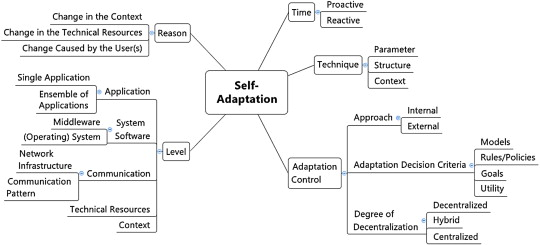
\includegraphics[width=\textwidth]{images/KrupitzerTaxonomy.jpg}
    \caption{Taxonomy for \acrlong{sas}[s] by Krupitzer et al., 2015 \cite*{SurveyOnEngineeringApproaches}}
    \label{fig:KrupitzerTaxonomy}
\end{figure*}

\noindent The taxonomy for \acrlong{sas}[s] by Krupitzer's et al., 2015 \cite*{SurveyOnEngineeringApproaches} in Figure \ref{fig:KrupitzerTaxonomy}
is based upon the 5W+1H questions by Salehie and Tahvildari, 2009 \cite*{LandscapeAndResearchChallenges}.
These questions are: Where, When, What, Why, Who and How.
Each of these questions is responsible for a different aspect of \acrlong{sas}[s] and corresponds to a dimension of the taxonomy.

\subparagraph*{Why}
First there needs to be a reason for a Self-Adaptive System to adapt. Why an adaptation should be performed is answered by the Reason dimension.
According to the taxonomy reasons for an adaptation can be changes in either the context, a technical resource or changes caused by the user.

\subparagraph*{Where}
The question of where asks on which level of the system changes need to occur.
The different levels on which changes can occur include:
\begin{itemize}[nosep]
    \item Different levels of applications from the operating system to a user application.
    \item How systems communicate with each other.
    \item The technical resources that are needed by the system.
    \item The context in which the system operates.
\end{itemize}

\subparagraph*{When}
While the original When-Question by Salehie and Tahvildari tries to understand all temporal aspects of \acrlong{sas}[s],
including how frequently changes should occur and if they happen continously,
the taxonomy only answers the question when changes should be performed.
For this purpose the Time dimension differentiates between systems that perform changes proactively or reactively.

\subparagraph*{What}
In addition to the question of where and when changes should occur, it is also important to know
what changes should occur. There are different techniques that can be used.
The Technique dimension of the taxonomy differentiates between systems that change parameters, their structure or their context.

\subparagraph*{Who}
After answering where, when, what and why changes should be performed, 
it is necessary to select who is responsible for these changes.
According to Salehie and Tahvildari it is also important to establish if the changes can be performed fully autonomous
or if the involvement of human operators is necessary.
The taxonomy does not directly address all of these concerns but states that:
"N/A (nature of a SAS leads to an automatic type of adaptation)" (Krupitzer et al., 2015 \cite{SurveyOnEngineeringApproaches}).

\subparagraph*{How}
Lastly, after determining the where, when, what, why and by who, there needs to be a way
to perform the required changes. This is answered by asking how the changes should be performed
and corresponds to the Adaptation Control.
The three main factors of the Adaptation Control are the degree of decentralization, the adaptation decision criteria
and the approach taken by the system, which divides \acrlong{sas}[s] into those where the adaptation logic is part of the application logic
and those with separated adaptation and application logic.

\noindent After classifying \acrlong{sas}[s] the following question can be asked: Which parts of a Self-Adaptive System can be optimized?
To answer this we will start by looking at which parts can not be optimized or do not benefit from optimization.

\noindent The first part that can not be optimized is the environment which provides the Reason dimension.
While the environment for a Self-Adaptive System can be chosen in a way which is most beneficial for the system
and can be influenced by actors,
the behavior of the systems environment can generally not be controlled completely.

\noindent Another dimension of \acrlong{sas}[s] that can not be optimized, or is not useful to optimize,
is the Time dimension. This dimension is mostly a design decision on how the system should behave and be constructed.
It is also a question of how to handle uncertainty and the level of accepted risk.
A proactive system can prevent faults and degradation in Quality-of-Service metrics,
but it can also predict the wrong changes which can lead to a situation where the system itself generates faults by
reacting in a way that is contradictive to its goals.
A reactive system can not prevent faults like a proactive system,
but its behavior can be much more stable, because it only has to react to a change and not predict that change as well.

\noindent Lastly, the question of who is responsible can not be optimized, because the taxonomy simply answers it,
by referring to the name "Self-Adaptive System" which implies that the system itself is responsible for managing adaptations.

\noindent The three remaining dimensions can be optimized or can benefit from being adapted dynamically.
These are the Adaptation Control, the Level and the Technique.

\noindent The Approach and the Degree of Decentralization used by the Adaptation Control can not be optimized 
because they are design decisions of how the system is built.
However, the Adaptation Decision Criteria can be optimized. An optimization of the Adaptation Decision Criteria
could, for example, be to dynamically adapt the rules and policies at runtime to better reflect a changing environment.

\noindent Another dimension that can be optimized is the Technique. 
This can be optimized by changing what gets adapted by the system.

\noindent The last dimension that can be optimized is the Level, which can be done by dynamically changing at which level of the system
adaptations should be performed.

\noindent This explanation of how \acrlong{sas}[s] are classified,
leads us to how we can classify Optimization Approaches for \acrlong{sas}[s].
The main concepts that will be used for the classification of Optimization Approaches are:
\begin{itemize}[nosep]
    \item The concept of reflectiveness as a way to model self-adaptation.
    \item The 5W+1H questions to determine how a Self-Adaptive System operates.
    \item The MAPE-K feedback loop a general base for understanding \acrlong{sas}[s].
    \item The concept of self-* properties which enables us to differentiate between self-adaptation
    and other self-* abilities.
    \item A taxonomy for \acrlong{sas}[s] which will be the basis for the proposed classification of Optimization Approaches,
    because \acrlong{sas}[s] are so closely related to their Optimization Approaches.
\end{itemize}